\chapter{CBIR Overview}

  \section{Introduction}

    It is often said that an image is worth a thousand words. This idiom refers to the notion that a complex idea can be conveyed with just a single still image. Indeed they are a powerful mean of communication and we interact with them in our everyday life. We use them to freeze a moment and share it with our relatives and friends, to illustrate a written article or to capture a emotion in a painting. Nowadays an increasing number of devices, cameras, satellites, video sensors, allow us to automatically record digital images which are then stored in constantly increasing databases. The phenomenal expansion of the web enabling us to store those images online also contributes to this collection of images in very huge databases. To allow us to take advantage of this increasing amount of data we need to develop tools that efficiently process images and retrieve them in a meaningful fashion. This is the problem addressed by Content-Based Image Retrieval. Formally it can be defined as \textit{any technologies that help to deal with the organization of digital pictures based on their content} \cite{CBIR_Trends_NewAge}. The key idea is that no metadata is involved and only the raw pixels of the images are used in order to infer semantic knowledge. It is a growing field which span over numerous research area such as Information Retrieval, Computer Vision, Machine Learning...

    Humans are naturally gifted to deduce informations by just looking a few seconds at an image and it is interesting to understand how we are performing this task in order to be able to reproduce it into a machine. In doing this operation we are usually relying on at least three different factors :

    \begin{description}
      \item[Our sensory abilities] Our sensory abilities refer to our ability to acquire visual inputs through our eyes and the process that is made of these inputs by our visual cortex.

      \item[The context] The context of an image include everything that is not in the image but contribute to its interpretation. It is well known that an image can have different meaning depending on its context.

      \item[Our experiences] Different experiences makes us respond differently when confronted to an situation. This is valid for the interpretation of an image which will rationally differ between individuals.

    \end{description}

    In order to successfully retrieve images for an end-user a machine should theoretically be able to incorporate these three factors into its process. As one can imagine such objective is especially challenging for many reasons. First we are far from completely understanding how our brain is processing the visual inputs that it receives. Then the context of an image is not always available, especially when dealing only with raw pixels without the help of additional metadata. Finally individuals with different cultures can have very different interpretation of the same image and retrieve the right images for an user would imply to hame some knowledge about its background or intentions.

  \section{Real World Applications}

  Even if the process of making good interpretation based on the content of an image is far from being mastered
  numerous real world applications make already use of Content-Based Image Retrieval technologies. Among this different applications we can already differentiate between those who operate on images with a very broad domain and those who operate on a narrow domain. In the review made by Smeulders and all \cite{smeulders2000content} they define a broad domain as having \textit{"an unlimited and unpredicted variability even for the same semantic meaning"}. Web applications and general visual search engine often process on a broad domain since images can come from many different users and similar objects can have different size, shape or illumination and can even be partially occluded.

  The first visual search engine was developed by IBM with their commercial system called QBIC (Query by Image Content)\cite{QBIC}. QBIC enable an user to query a image database with image queries. Many possibilities is given to the user to specify its query. He can either query by sketch, query by specifying specific color, texture and shape or query using an image similar to the ones he was looking for. Depending on the type of the query different similarities measures are then used to retrieve the most similar images. In order to help further the research semi-automatic detection of object or point of interest is also performed when a new image is inserted into the database. Since this first attempt other systems (TinEye, Pinterest, Google Query By Image) have been developed which rely on more advanced techniques. For instance Pinterest is a web and mobile applications where user can upload images of interest through collections known as pinboards. Pinterest then use those images to look for similar images and recommend them to the user. While QBIC was only relying on handcrafted features Pinterest, among other algorithms, rely on features learning and algorithms called Convolutional Neural Network to extract features from images \cite{jing2015visual}.

  As opposed to a broad domain a narrow domain is defined as having \textit{a limited and predictable variability in all relevant aspects of its appearance}. When dealing with a narrow domain knowledge of the domain can be efficiently used to design good features detectors. Illustration of a narrow domain can be found in many applications such as medical diagnosis or face recognition. In the medical domain, due in part to the steadily growing rate of image production, Content-Based Image Retrieval can play a key role in many medical applications\cite{muller2004review}. It can for example enable the automatic annotation and the classification of medical images. Content-Based Image Retrieval can also be used to help in the clinical decision–making process. Indeed when confronted with a medical case an useful scenario would be to supply the doctor with similar cases by finding other images of the same disease that would allow him to take a decision with more informations at hand. Another application is for instance within the radiology department to develop tools that enable automatic diagnostic of the diseases \cite{kahn1994artificial}.

  % Find other domain (check Content-Based Image Retrieval Systems )

  % Techniques from content-based image retrieval are already all around us. For example automatic face recognition of our friends on Facebook use ...

  Content-Based Image Retrieval techniques might also find useful applications in many more domains. For instance in digital art gallery or museum collection available online they can be used to bring to the user art work similar to the ones he browsed. For law enforcement and criminal investigation they could help investigator to process pictures of security cameras.

    % Applications of Content-Based Image Retrieval is of course not limited to the ones illustrated above and as the field
    % become more mature we can expect that more and more applications will emerge.

  \section{Components of CBIR systems}

    All typical Content-Based Image Retrieval systems are usually performing common steps to achieve the retrieval of images as illustrated by the figure \ref{pipeline}. The first steps which might be performed is segmentation which can be useful to isolate meaningful regions from the background for example. As a second step features extraction is performed. The extraction of features can rely of two different methods. Either it is done through handcrafted features that is humans have to design a specific features detector for the problem at hand or it is done through feature learning that is we let the machine learn features thanks to training samples. In the domain of image processing one model have started to show great promises to learn features and is known as Convolutional Neural Network. One of the great challenge of features extraction is to reduce what is known as the \textit{semantic gap} that is the difference between the interpretation of the image and the features that have been computed. Finally one have to interpret these features which is often done through a similarity measure or a machine learning classifier. The following of this work will detail each of these steps.

    \begin{figure}[H]
      \centering
        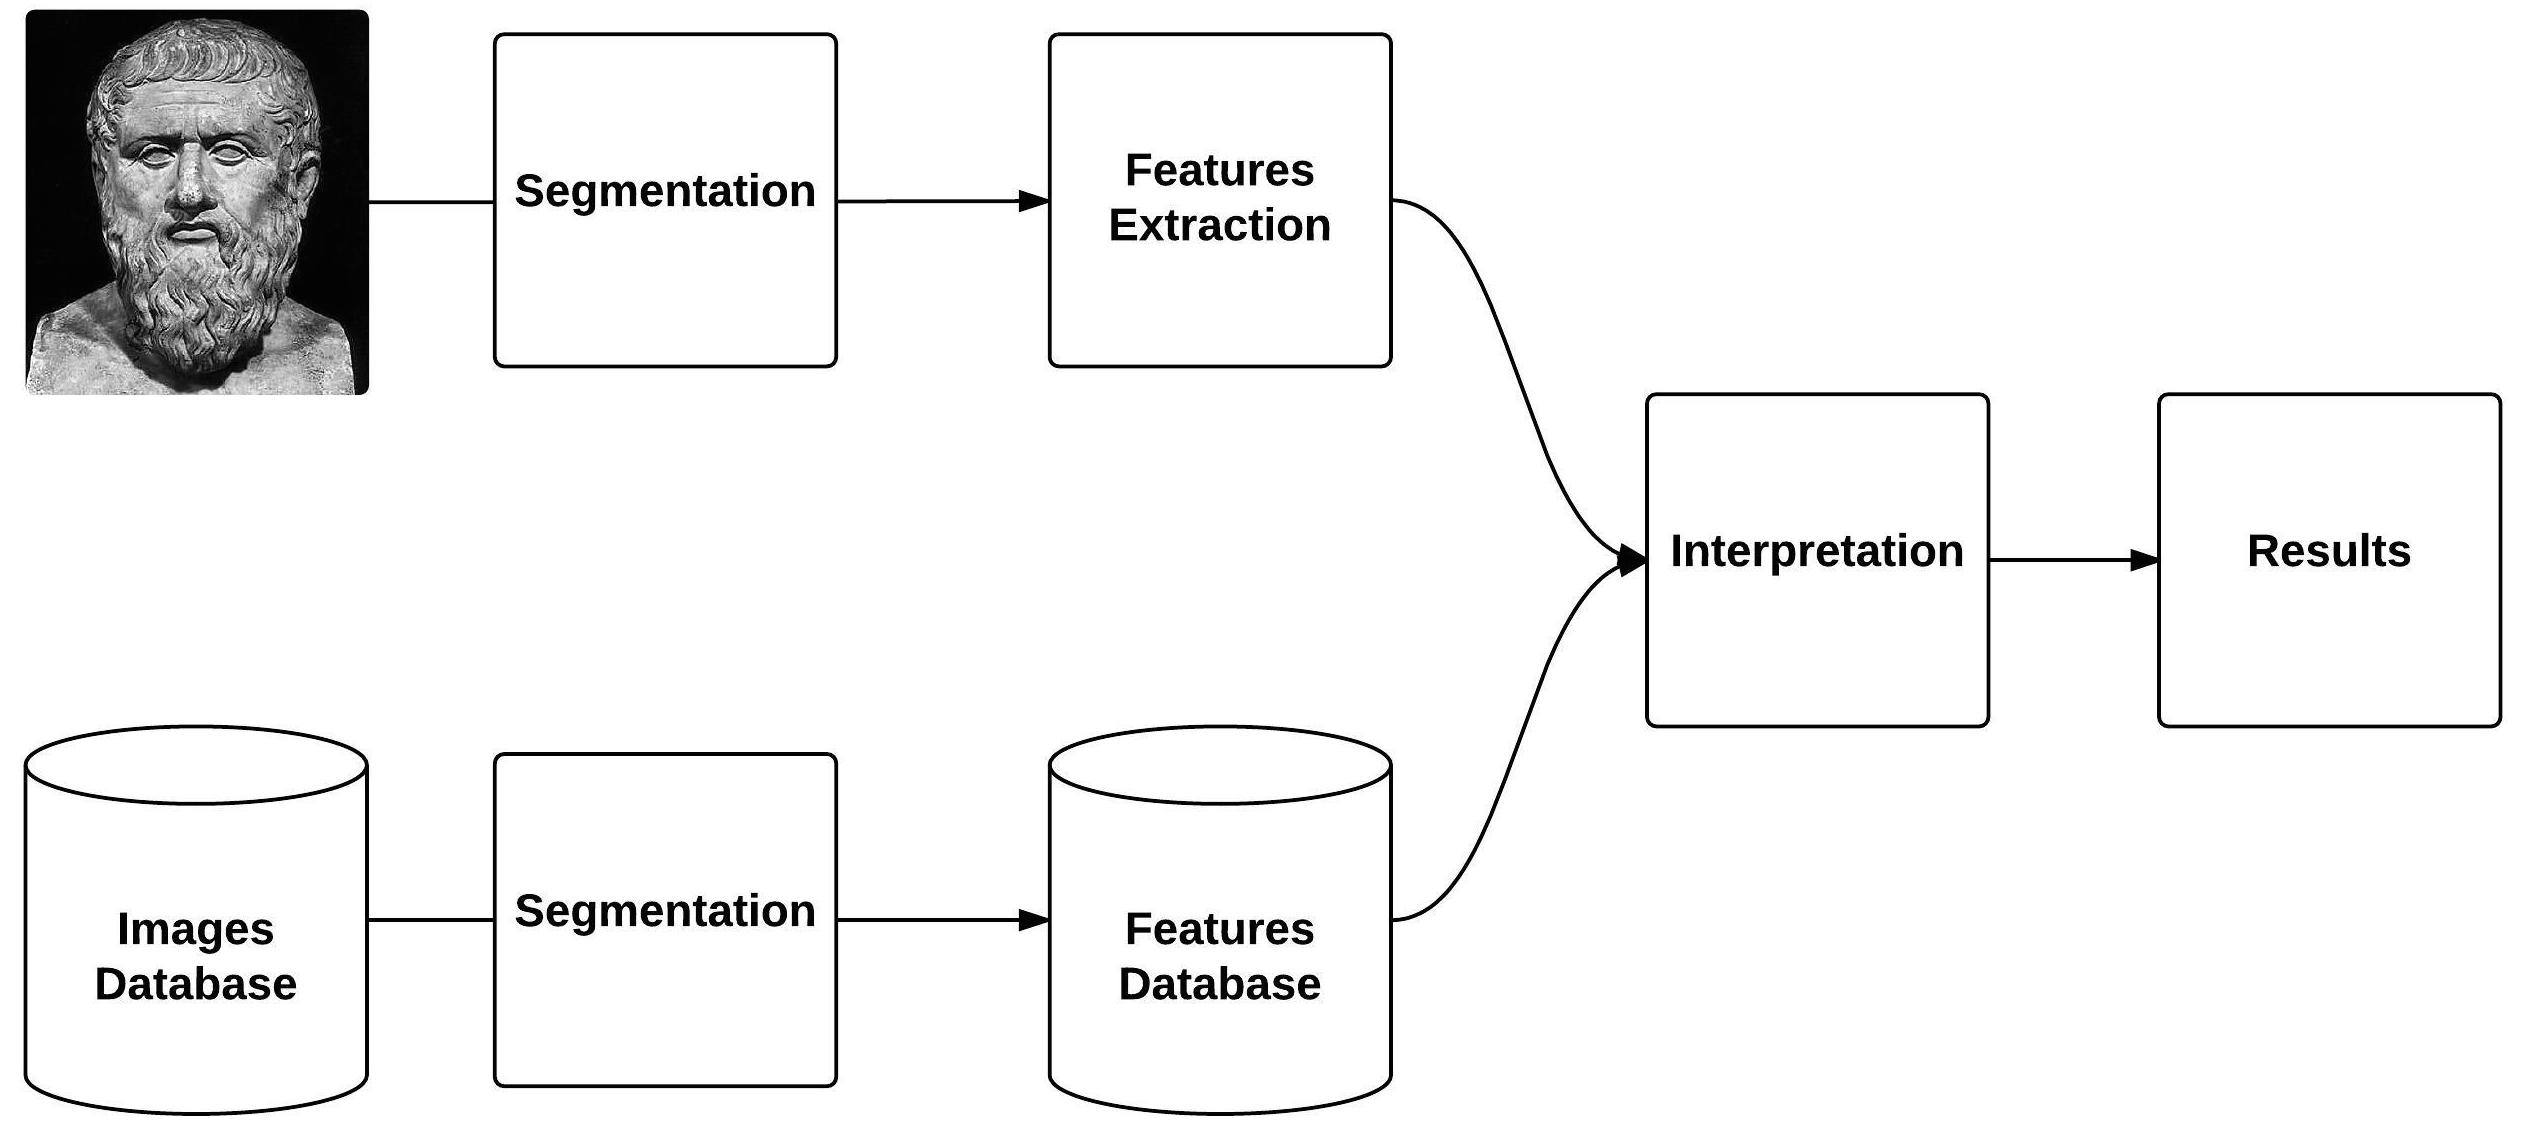
\includegraphics[width=1\textwidth]{images/cbir_pipeline.jpeg}
      \caption{Content-Based Image Retrieval System Components}
      \label{pipeline}
    \end{figure}

    While every Content-Based Image Retrieval system usually perform the operations described above their performance is not limited to them. Below is a review of the main components that typically compose a CBIR systems and improvement in each of these components is required to achieve better systems \cite{gudivada1995content}.

    \subsection{Database Management}

      When an image database is growing very large efficient access methods should be developed in order to speed up the retrieval of images. These methods should act as a filter with only relevant images being retrieved from the storage system and tested for similarity with the query image. Most data structure used today for indexing are spatial access methods and assume that all images features are numeric and represent an image as a point in a multidimensional space. These methods can be classified into three categories : \textit{space partitioning}, \textit{data partitioning} an \textit{distance-based} techniques \cite{smeulders2000content}. Space partitioning techniques (k-d tree, k-d B-tree...) organize the feature space as a tree and with a node standing for a region of the space. When a region contain too much points it is split in subregions whose nodes become the children of the original regions. Data partitioning techniques (R-tree,  R+-tree, R*-tree...) associate with each points a region representing the neighborhood of that point and leaf nodes correspond to minimum bounding regions of a set of vectors. Distance-Based index structures (VP-tree, MVP-tree, M-tree...) is applicable to general metric spaces whose primary idea is to pick an example point and divide the rest of the features space into concentric rings around the example. Nevertheless when the features vectors being indexed contain a considerable number of dimensions the performance of the previous indices greatly decrease. This is known as the \textit{curse of dimensionality} phenomenon.

    \subsection{Query Specification}

      Queries made by the user can take several forms which logically influence on the retrieval process. Query by example where the user provide a image and similarity is computed based on the entire scene is a common way to perform the request Another method is to let the user specify a region of interest (a person or an object for example) and search for images with similar regions. Yet an other way is for the user to draw a sketch of the item or landscape he is interested in.
      How the query is specified depend of the users of the system. Casual users surely prefer to make its request by using natural language \say{Find me mountain with snow and with a bird in the sky} or with an image as an example whereas domain expert might want more sophisticated methods such as query by sketch.

    \subsection{Relevance Feedback}

      As pointed out earlier bringing relevant images to the end user imply to know its point of view. Learning the point of view of the user is more and more achieved through relevant feedback. From a broad perspective a relevance feedback scenario usually has the following scheme. First initial results are returned by the machine then the user provide a judgement on the results being displayed and finally the machine learns from the judgement to retrieve new results and so on. The exact algorithm used for learning is going to depend on whether the user is looking on a particular target item or a class of similar item. Also it is going to differ if the user provide a binary judgement (relevant or not) or a comparative judgement (this result is better that this one). Different relevance feedback algorithms can be found in the survey of Zhou and all \cite{zhou2003relevance} or the one of Crucianu and all \cite{crucianu2004relevance}.
